\subsection{Pipeline Steps}\label{HiC:index} %index
Within the parent directory of an analysis, the default pipeline steps are listed as symlinks, in alpha-numeric order starting with "\_\_", as seen here:


\begin{lstlisting}
lrwxrwxrwx  1 at570  14 Feb  7 17:06 __01a-align -> pipeline/align
lrwxrwxrwx  1 at570  15 Feb  7 17:06 __02a-filter -> pipeline/filter
lrwxrwxrwx  1 at570  21 Feb  7 17:06 __02b-filter-stats -> pipeline/filter-stats
lrwxrwxrwx  1 at570  15 Feb  7 17:06 __03a-tracks -> pipeline/tracks
lrwxrwxrwx  1 at570  24 Feb  7 17:06 __04a-matrix-filtered -> pipeline/matrix-filtered
lrwxrwxrwx  1 at570  20 Feb  7 17:06 __05a-matrix-prep -> pipeline/matrix-prep
lrwxrwxrwx  1 at570  18 Feb  7 17:06 __06a-matrix-ic -> pipeline/matrix-ic
lrwxrwxrwx  1 at570  23 Feb  7 17:06 __07a-matrix-hicnorm -> pipeline/matrix-hicnorm
lrwxrwxrwx  1 at570  21 Feb  7 17:06 __08a-matrix-stats -> pipeline/matrix-stats
lrwxrwxrwx  1 at570  25 Feb  7 17:06 __09a-compare-matrices -> pipeline/compare-matrices
lrwxrwxrwx  1 at570  31 Feb  7 17:06 __09b-compare-matrices-stats -> pipeline/compare-matrices-stats
lrwxrwxrwx  1 at570  24 Feb  7 17:06 __10a-boundary-scores -> pipeline/boundary-scores
lrwxrwxrwx  1 at570  28 Feb  7 17:06 __10b-boundary-scores-pca -> pipeline/boundary-scores-pca
lrwxrwxrwx  1 at570  16 Feb  7 17:06 __11a-domains -> pipeline/domains
lrwxrwxrwx  1 at570  27 Feb  7 17:06 __12a-compare-boundaries -> pipeline/compare-boundaries
lrwxrwxrwx  1 at570  33 Feb  7 17:06 __12b-compare-boundaries-stats -> pipeline/compare-boundaries-stats
lrwxrwxrwx  1 at570  19 Feb  7 17:06 __13a-hicplotter -> pipeline/hicplotter
lrwxrwxrwx  1 at570  21 Feb  7 17:06 __14a-interactions -> pipeline/interactions
lrwxrwxrwx  1 at570  20 Feb  7 17:06 __15a-annotations -> pipeline/annotations
lrwxrwxrwx  1 at570  30 Feb  8 17:47 code -> code.repo/code.hicseq-standard
lrwxrwxrwx  1 at570  14 Nov 12 11:55 code.main -> code/code.main
drwxr-xr-x  9 at570 209 Jan  9 10:16 code.repo
lrwxrwxrwx  1 at570 103 Feb  8 17:47 data -> /ifs/home/.../data
drwxr-xr-x  6 at570 258 Jan  5 09:24 inputs
drwxr-xr-x 24 at570 799 Feb  7 17:06 pipeline
-rwxr-xr-x  1 at570 210 Dec  2 14:23 psync
-rwxr-xr-x  1 at570 981 Jan  5 19:40 run
-rwxr-xr-x  1 at570 554 Dec 18 17:02 run.dry
-rwxr-xr-x  1 at570 988 Jan 24 14:42 run.subset
-rwxr-xr-x  1 at570 165 Dec 26 08:09 run.usage
\end{lstlisting}

This functions in informing the user of the order of pipeline steps. Each symlink points back to a directory in the pipeline directory for the corresponding pipeline step, as shown here:


\begin{lstlisting}
pipeline$
total 814K
drwxr-xr-x  4 at570 203 Jan 19 15:50 align
drwxr-xr-x  5 at570 207 Jan 19 22:12 annotations
drwxr-xr-x  5 at570 387 Feb  6 17:46 boundary-scores
drwxr-xr-x  5 at570 243 Feb  7 14:17 boundary-scores-pca
lrwxrwxrwx  1 at570   7 Dec  2 12:39 code -> ../code
lrwxrwxrwx  1 at570  12 Dec  2 12:39 code.main -> ../code.main
drwxr-xr-x  5 at570 390 Jan 19 22:08 compare-boundaries
drwxr-xr-x  5 at570 396 Jan 20 10:59 compare-boundaries-stats
drwxr-xr-x  5 at570 435 Jan 19 16:04 compare-matrices
drwxr-xr-x  6 at570 419 Jan 19 16:05 compare-matrices-stats
drwxr-xr-x  5 at570 445 Jan 19 22:10 diff-domains
drwxr-xr-x  5 at570 379 Jan 20 13:06 domains
drwxr-xr-x  5 at570 229 Jan 19 16:19 filter
drwxr-xr-x  6 at570 256 Jan 19 15:53 filter-stats
drwxr-xr-x  5 at570 206 Jan 19 22:11 hicplotter
-rw-r--r--  1 at570 297 Feb  6 17:52 index.txt
lrwxrwxrwx  1 at570   9 Dec  2 12:39 inputs -> ../inputs
drwxr-xr-x  5 at570 208 Jan 19 22:12 interactions
drwxr-xr-x  5 at570 239 Jan 19 16:01 matrix-estimated
drwxr-xr-x  5 at570 238 Jan 19 16:08 matrix-filtered
drwxr-xr-x  5 at570 232 Jan 19 16:00 matrix-ic
drwxr-xr-x  5 at570 234 Jan 19 15:59 matrix-prep
drwxr-xr-x  5 at570 208 Jan 19 16:03 matrix-stats
lrwxrwxrwx  1 at570   8 Dec  3 14:56 psync -> ../psync
drwxr-xr-x  4 at570 158 Dec 22 17:44 template
drwxr-xr-x  5 at570 229 Jan 19 15:55 tracks
\end{lstlisting}

The pipeline directory contains files and symlinks needed for each step in the pipeline. The steps to be exectuted are defined in two ways:
\begin{enumerate}
\item A file called 'index.txt' lists the names of each step in the pipeline, in the order in which they will be completed. This file is located in the 'pipeline' directory. 
\item A subdirectory within the 'pipeline' directory with the same name as its corresponding entry in the 'index.txt' file must be included to hold the parameters and commands to be run, and the results produced. 
\end{enumerate}

Index file:
\begin{lstlisting}
pipeline/index.txt$ 
align

filter
filter-stats

tracks

matrix-filtered

matrix-prep

matrix-ic

#matrix-estimated
#
matrix-stats

compare-matrices
compare-matrices-stats

boundary-scores
boundary-scores-pca

domains

compare-boundaries
compare-boundaries-stats

#diff-domains
#
hicplotter

interactions

annotations
\end{lstlisting}

Steps listed in 'index.txt' which have been commented out (i.e. start with a \# character) will not be included in the analysis. Custom pipeline steps can be easily included by adding the corresponding entry to the 'index.txt' and creating a subdirectory within the 'pipeline' directory. 

For details on adding custom pipeline steps, see Section~\ref{custom-pipeline-step}
%~~~~~~~~~~~~~~~~~~~%
\subsubsection{Default Parameters}\label{HiC:default-params}
These parameters are used by default across pipeline steps.

\begin{lstlisting}
/inputs/params/params.tcsh$
#!/bin/tcsh

# load basic tools
module unload samtools
module unload java
module unload gcc
module unload python
module load samtools/1.2.1
module load bedtools/2.22.0
module load java/1.7
module load picard-tools

# load tools required for each step of the pipeline (this can be overriden in local param scripts)
module load bowtie2/2.2.6
module load armatus/2014-05-19
module load caltads/0.1.0
module load ghmm/0.9

# sample sheet file
set sheet = inputs/sample-sheet.tsv
\end{lstlisting}
%~~~~~~~~~~~~~~~~~~~%
\subsubsection{Pipeline Step Execution Flowchart}\label{HiC:pipeline-flowchart}
\begin{figure}[!htb]
    \centering
%     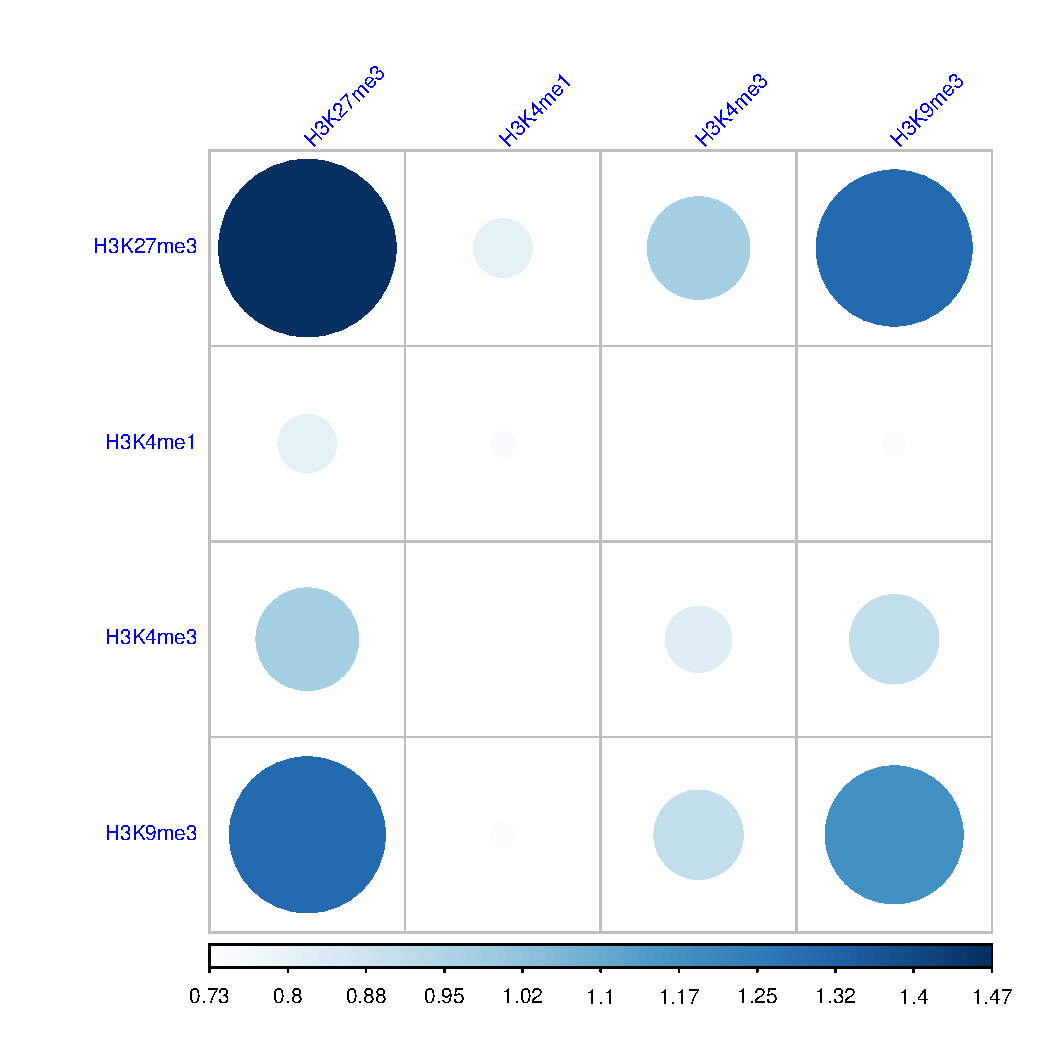
\includegraphics[width=\textwidth,height=0.5\textheight,keepaspectratio]{figure/annotations-stats_enrichment}
    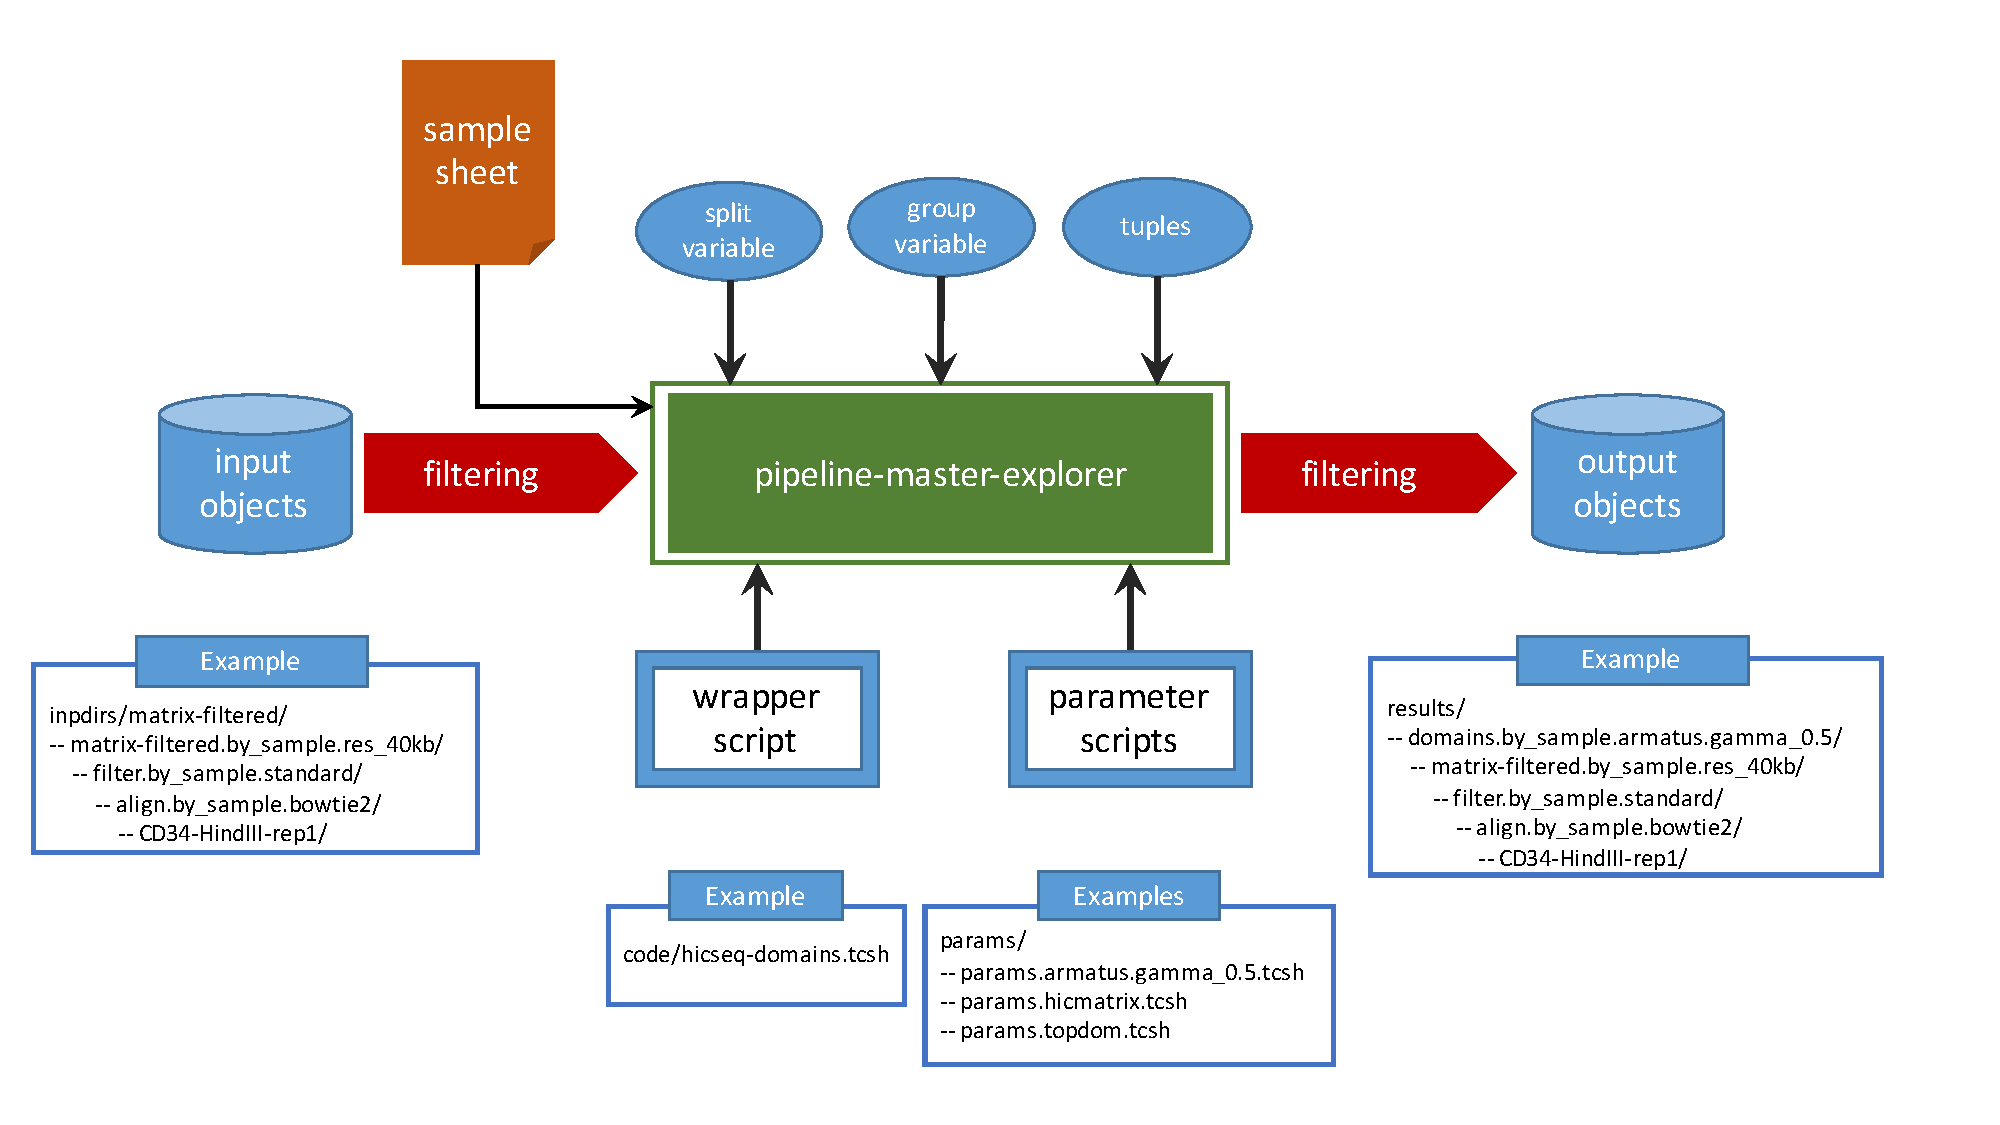
\includegraphics[width=\textwidth,height=\textheight,keepaspectratio]{figure/HiC_flowchart_Figure_2}
    \caption{Overview of pipeline step execution for default analysis steps. See Section~\ref{HiC:pipeline-flowchart}.} % results/annotations-stats.by_sample.standard/annotations.by_sample.standard/interactions.by_sample.standard/matrix-filtered.by_sample.res_10kb.maxd_5Mb.rotate45/filter.by_sample.standard/align.by_sample.bowtie2/CD34-HindIII-rep1/enrichment.pdf
    \label{fig:pipeline-flowchart}
\end{figure}
% \newpage
\clearpage